% ============================================================
%  Biomimetic Pipeline — Architecture & Operations Guide
%  Ready for Overleaf (pdflatex)
% ============================================================
\documentclass[11pt, letterpaper]{article}

% ── Encoding & fonts ────────────────────────────────────────
\usepackage[T1]{fontenc}
\usepackage[utf8]{inputenc}
\usepackage{lmodern}
\usepackage{microtype}

% ── Page geometry ───────────────────────────────────────────
\usepackage[top=1in, bottom=1in, left=1.1in, right=1.1in]{geometry}

% ── Math ────────────────────────────────────────────────────
\usepackage{amsmath, amssymb}

% ── Graphics & colour ───────────────────────────────────────
\usepackage{graphicx}
\usepackage[dvipsnames, table]{xcolor}

% ── Tables ──────────────────────────────────────────────────
\usepackage{booktabs}
\usepackage{array}
\usepackage{multirow}
\usepackage{tabularx}
\usepackage{longtable}

% ── Lists ───────────────────────────────────────────────────
\usepackage{enumitem}
\setlist[itemize]{leftmargin=1.6em, topsep=3pt, itemsep=2pt}
\setlist[enumerate]{leftmargin=1.6em, topsep=3pt, itemsep=2pt}

% ── Section formatting ──────────────────────────────────────
\usepackage{titlesec}
\titleformat{\section}{\large\bfseries\color{NavyBlue}}{{\thesection.}}{0.5em}{}[\vspace{-4pt}\rule{\linewidth}{0.4pt}]
\titleformat{\subsection}{\normalsize\bfseries\color{MidnightBlue}}{\thesubsection}{0.5em}{}
\titleformat{\subsubsection}{\normalsize\itshape\color{black}}{\thesubsubsection}{0.5em}{}

% ── Highlighted conclusion boxes ────────────────────────────
\usepackage{tcolorbox}
\tcbuselibrary{breakable, skins}

\newtcolorbox{conclusionbox}[1]{
  breakable,
  colback=NavyBlue!5!white,
  colframe=NavyBlue!60!white,
  fonttitle=\bfseries\small,
  title={#1},
  left=4pt, right=4pt, top=3pt, bottom=3pt,
  boxrule=0.6pt,
}

\newtcolorbox{limitbox}{
  breakable,
  colback=BrickRed!5!white,
  colframe=BrickRed!50!white,
  left=4pt, right=4pt, top=3pt, bottom=3pt,
  boxrule=0.6pt,
}

\newtcolorbox{mechanismbox}{
  breakable,
  colback=gray!6!white,
  colframe=gray!50!white,
  fonttitle=\bfseries\small,
  left=4pt, right=4pt, top=3pt, bottom=3pt,
  boxrule=0.5pt,
}

% ── Code / verbatim ─────────────────────────────────────────
\usepackage{listings}
\lstset{
  basicstyle=\ttfamily\footnotesize,
  backgroundcolor=\color{gray!10},
  frame=single, framesep=3pt,
  breaklines=true,
  xleftmargin=6pt, xrightmargin=6pt,
  columns=fullflexible,
  keepspaces=true,
}

% ── Hyperlinks ──────────────────────────────────────────────
\usepackage[colorlinks=true, linkcolor=NavyBlue,
            urlcolor=NavyBlue, citecolor=NavyBlue]{hyperref}
\hypersetup{
  pdftitle={Biomimetic Pipeline: Architecture \& Operations Guide},
  pdfauthor={Cameron Renteria},
  pdfsubject={Feature-driven CAD, load-normalized FEA, and closed-loop biomimicry for decussated enamel lattices},
  pdfkeywords={microCT, enamel, biomimetic, CAD, FEA, crack deflection, digital twin, SLA},
}

% ── Header / footer ─────────────────────────────────────────
\usepackage{fancyhdr}
\pagestyle{fancy}
\fancyhf{}
\rhead{\small Biomimetic Pipeline $\cdot$ Architecture \& Operations}
\lhead{\small Arola Lab $\cdot$ UW MSE}
\rfoot{\small\thepage}
\lfoot{\small April 14, 2026}
\renewcommand{\headrulewidth}{0.4pt}

% ── Paragraph spacing ───────────────────────────────────────
\usepackage{parskip}
\setlength{\parskip}{5pt}
\setlength{\parindent}{0pt}

% ── Misc ────────────────────────────────────────────────────
\usepackage{textcomp}
\usepackage{siunitx}
\sisetup{detect-all, separate-uncertainty=true}

% ============================================================
\begin{document}
% ============================================================

% ── Title page ──────────────────────────────────────────────
\begin{titlepage}
  \centering
  \vspace*{1.2cm}

  {\color{NavyBlue}\rule{\linewidth}{1.5pt}}\\[0.8em]

  {\LARGE\bfseries Biomimetic Pipeline\\[0.4em]
   Architecture \& Operations Guide:\\[0.3em]
   Feature-Driven CAD, Load-Normalized FEA,\\[0.3em]
   and Closed-Loop Biomimicry for\\[0.3em]
   Decussated Enamel Lattices}\\[0.8em]

  {\color{NavyBlue}\rule{\linewidth}{1.5pt}}\\[1.6em]

  {\large\itshape An end-to-end digital-twin pipeline that ingests microCT morphometrics,\\[0.2em]
  drives parametric CAD and sfepy FEA, and closes the biomimicry loop\\[0.2em]
  by reverse-mapping high-objective designs to measurable biology.}\\[2em]

  \begin{tabular}{rl}
    \textbf{Report by:} & Cameron Renteria \\[4pt]
    \textbf{Affiliation:} & University of Washington, Materials Science \& Engineering (Arola Lab) \\[4pt]
    \textbf{Date:}      & April 14, 2026 \\[4pt]
    \textbf{Pipeline version:} & 0.1.0 \\[4pt]
    \textbf{Location:}  & \texttt{microct\_pipeline/biomimetic\_pipeline/} \\[4pt]
    \textbf{Upstream stack:} & \texttt{cad\_modeling/Decussated Models Continous Twist/} (wrapped, never modified) \\[4pt]
    \textbf{Conda envs:} & \texttt{cad\_env} (CadQuery) $\cdot$ \texttt{sfepy\_env} (Gmsh, sfepy) \\[4pt]
    \textbf{Objective (default):} & maximize \texttt{crack\_deflection\_tortuosity\_p90} at $\overline{\mathrm{VM}} = 200$\,MPa \\
  \end{tabular}

  \vfill

  {\small Every design is evaluated at a matched 200\,MPa representative von-Mises stress via an in-loop
  strain solver, so the crack-deflection, toughness, and biomimicry metrics compare designs on a load-normalized basis.}
\end{titlepage}

% ── Table of Contents ───────────────────────────────────────
\tableofcontents
\newpage

% ============================================================
\section{Executive Summary}
% ============================================================

This document describes \textbf{biomimetic\_pipeline}, a modular digital-twin system built on top of the existing microCT analysis stack and continuous-twist CAD generator at the University of Washington. The pipeline addresses a specific gap: measured morphometric features from microCT, PIV, and self-organising map (SOM) analyses exist in isolation, and the parametric lattice CAD model that was developed separately is driven by hand-picked parameters rather than by the biology itself. This pipeline closes that loop.

\begin{conclusionbox}{Three staged deliverables (all built on the same core)}
\begin{enumerate}
  \item \textbf{Digital twin per specimen} — measured morphometrics drive CAD parameters so the generated lattice statistically reproduces a specific microCT scan.
  \item \textbf{Fully parametric / stochastic population generator} — supports manual sweeps, distribution-sampled variants, and print-process manufacturability clamps (SLA first; $E \approx 2500$--$3500$\,MPa, minimum feature $\geq 0.3$\,mm).
  \item \textbf{Self-optimizing FEA loop} — pluggable objective (default: crack deflection). Closed-loop mode identifies which measured morphometric features produce high-objective lattices and writes them as \texttt{biomimicry\_targets.json}, a set of morphometric ranges to look for in real specimens.
\end{enumerate}
\end{conclusionbox}

\begin{mechanismbox}
\textbf{Operating point (load-normalized comparison).} Representative compressive stress is held at $\approx 200$\,MPa by bisecting the applied displacement — so every design is evaluated at the same load state. The strain required to reach that stress (\texttt{critical\_strain\_at\_200MPa}) is a first-class metric, alongside crack deflection, strain-energy density, stress-concentration factor, and specific toughness. This decouples objective quality from incidental stiffness differences.
\end{mechanismbox}

\begin{figure}[h!]
\centering
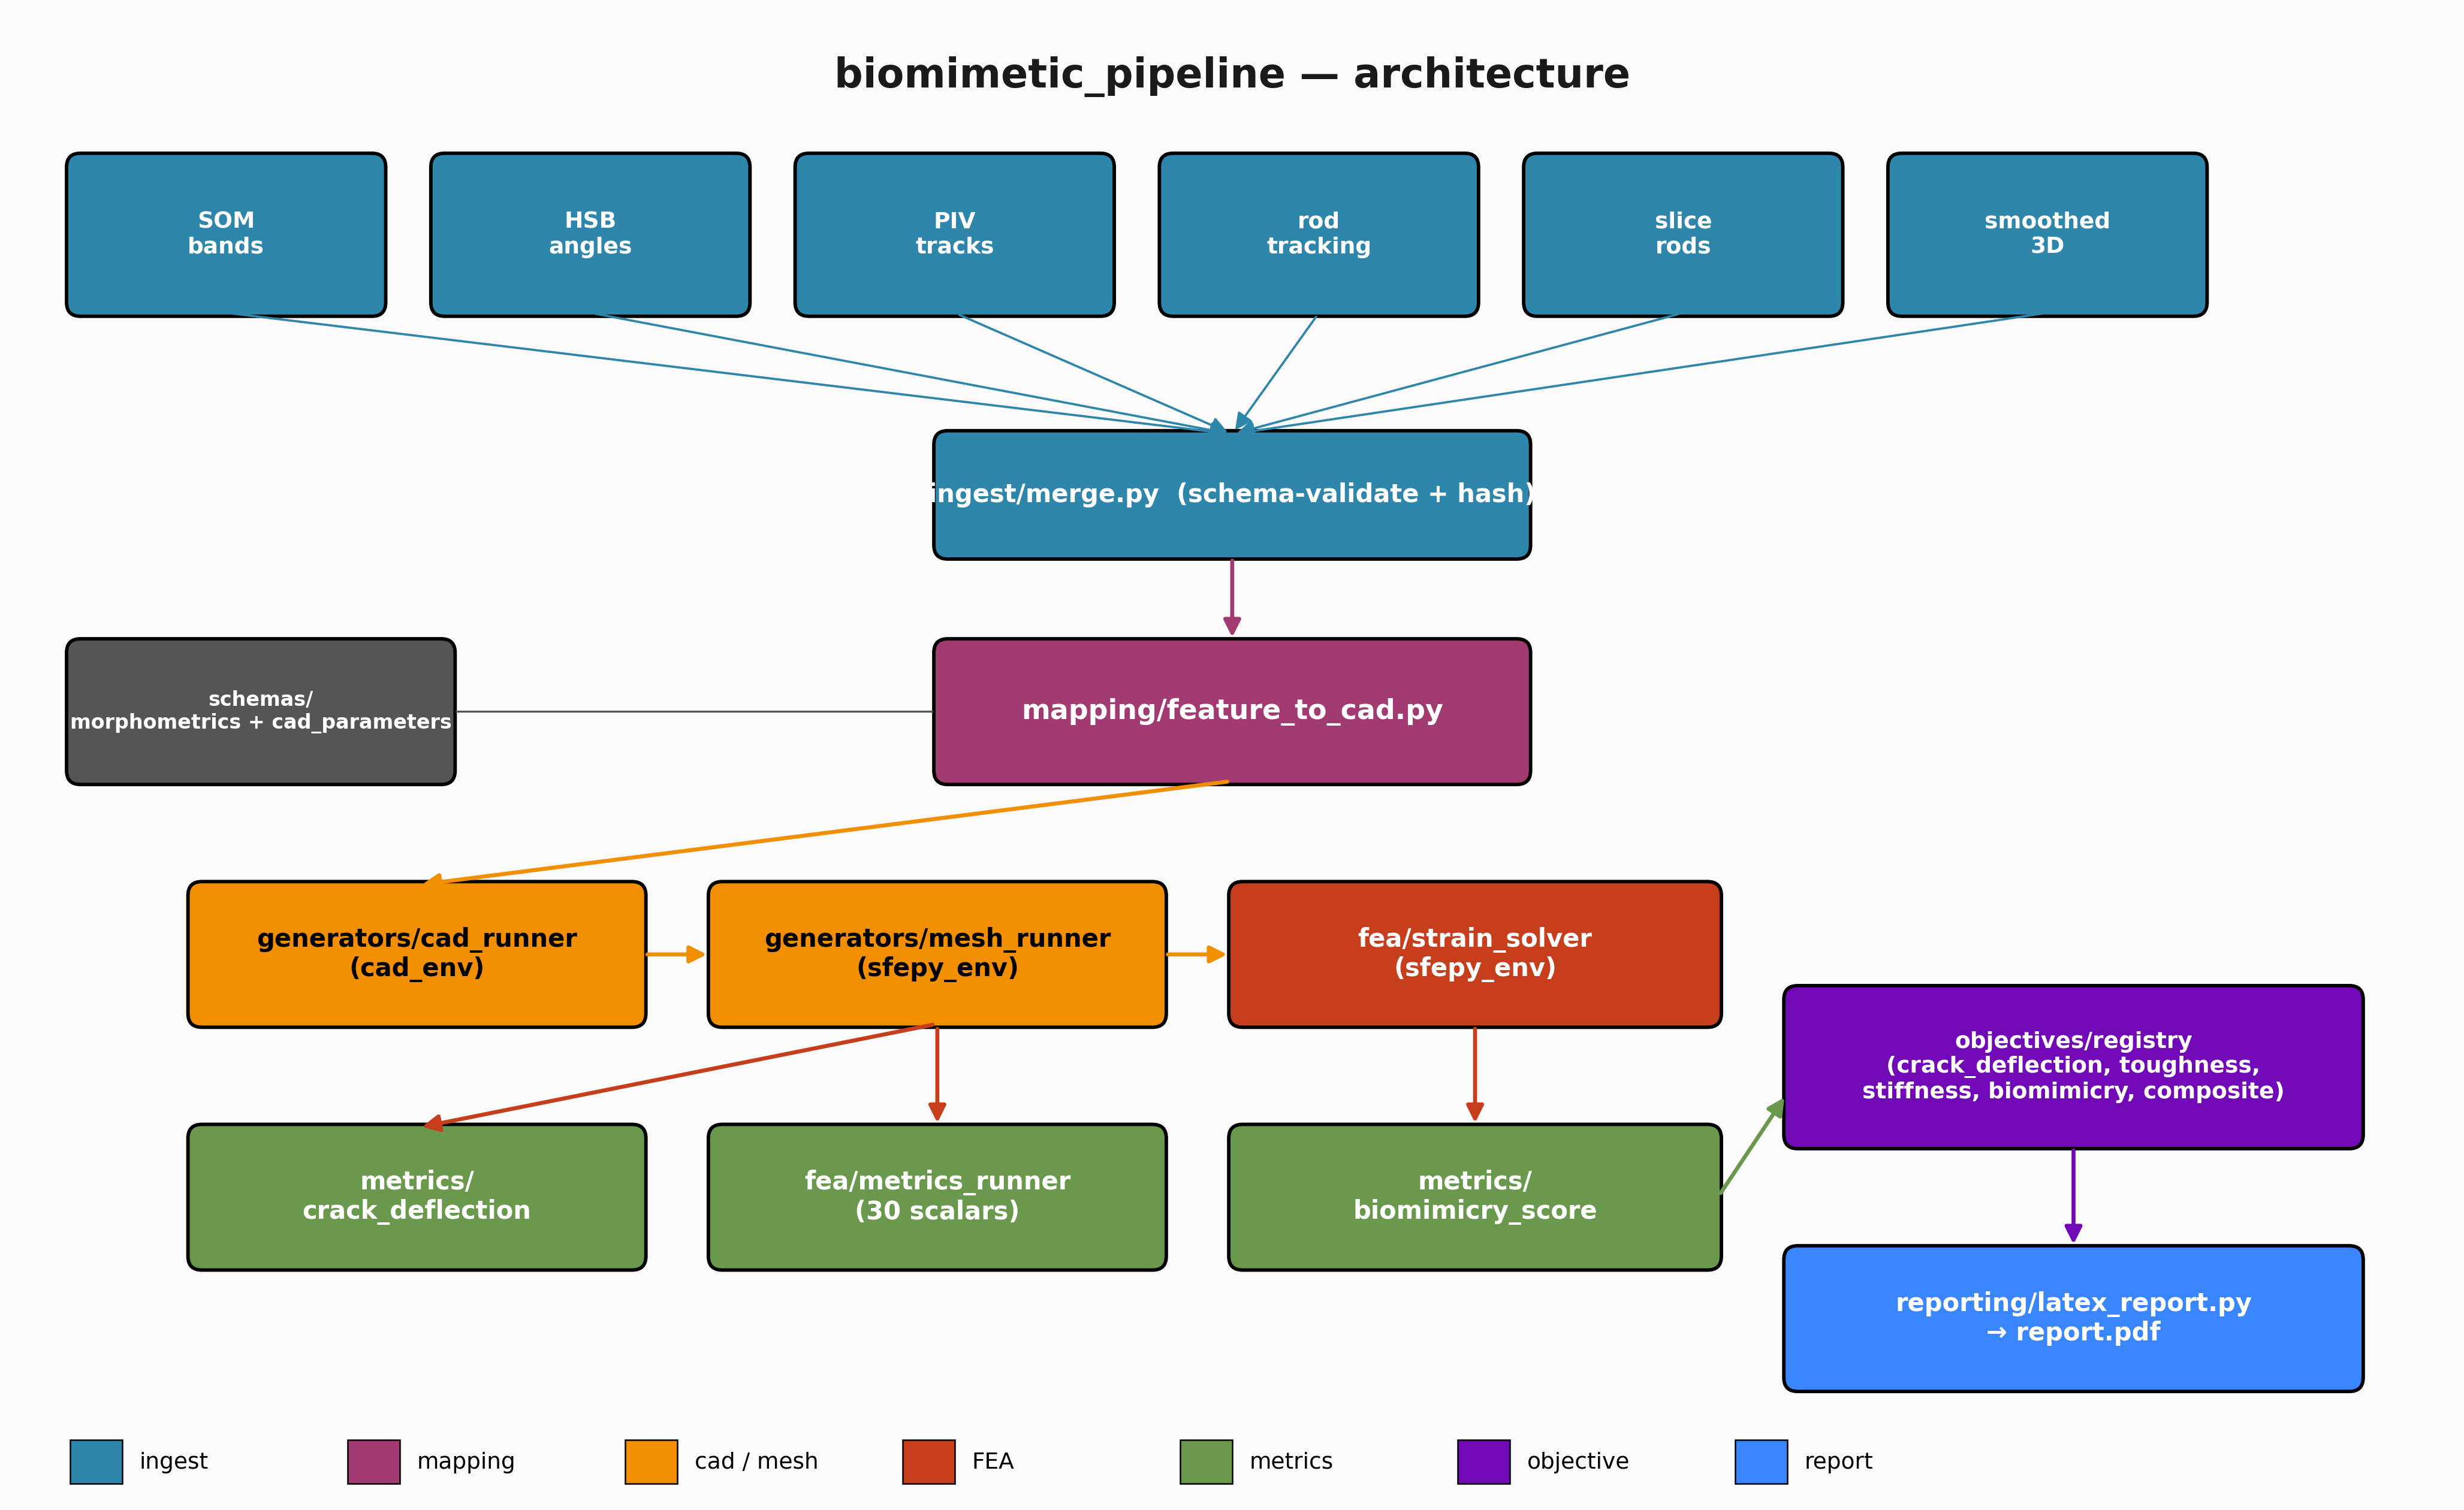
\includegraphics[width=0.95\linewidth]{figures/01_architecture.png}
\caption{Top-level architecture. Upstream outputs (blue) feed six ingesters into a canonical \texttt{morphometrics.json}. The mapping layer (magenta) produces \texttt{cad\_parameters.json}. CAD (orange) runs in \texttt{cad\_env}; mesh, FEA, and metrics extraction (red) run in \texttt{sfepy\_env}. The crack-deflection and biomimicry metrics (green) feed the pluggable objective (purple), which can drive parametric sweeps or Optuna-based optimisation. The LaTeX report (blue) closes the per-run loop.}
\label{fig:architecture}
\end{figure}

% ============================================================
\section{Design Principles}
% ============================================================

\subsection{Non-invasive wrapping}
Nothing inside \texttt{cad\_modeling/} is ever modified. The stock CadQuery \texttt{lattice\_cad.py}, the Gmsh \texttt{lattice\_mesh.py}, the sfepy problem definition \texttt{compression\_test.py}, and the metrics extractor \texttt{extract\_metrics.py} are all invoked via \texttt{conda\,run} with their existing CLI contracts intact. The pipeline supplies an auto-generated driver script that imports the stock CadQuery module as a library so full DEFAULTS control (including \texttt{RING\_ROTATION}, which is not exposed via CLI) is preserved without touching upstream code. The stock \texttt{lattice\_params.json} sidecar format is emitted by every model variant so \texttt{extract\_metrics.py} auto-detects bridge elevations and specimen geometry unchanged.

\subsection{Three canonical schemas}
Every stage hand-off is governed by a JSON Schema under \texttt{biomimetic\_pipeline/schemas/}:
\begin{itemize}
  \item \texttt{morphometrics.schema.json}: ingest $\to$ mapping; includes provenance (source paths, sha256 hashes, coordinate frame), depth profiles, angle statistics, SOM bands, periodicity, rod slice stats, and a track-tortuosity summary.
  \item \texttt{cad\_parameters.schema.json}: mapping $\to$ CAD; extends the stock DEFAULTS dict verbatim plus optional keys consumed only by new-model drivers (\texttt{measured\_twist\_profile}, \texttt{per\_ring\_diameter}, \texttt{rod\_cross\_section}, \texttt{biology\_scale\_factor}, \texttt{sla\_min\_feature\_mm}, \texttt{provenance}).
  \item \texttt{objective.schema.json}: YAML $\to$ pluggable scoring, with a \texttt{stress\_target} block that drives the strain solver.
\end{itemize}

\subsection{Biology-to-print scale + manufacturability clamps}
Measured rod diameter in real enamel is $\sim 4\,\si{\micro\meter}$; the stock continuous-twist reference geometry uses \texttt{ROD\_DIAMETER}\,$=2$\,mm, i.e. $\sim 500\times$ biological scale. That $500\times$ is the default \texttt{biology\_scale\_factor} so mapped lattices sit in the same SLA-printable regime as the stock model. A single source of truth in \texttt{mapping/scale.py} applies the scale factor and clamps every feature to \texttt{sla\_min\_feature\_mm} (default $0.3$\,mm). Every clamp is logged, with raw and clamped values, into \texttt{provenance.scale\_clamps} so the mapping is auditable.

\subsection{Lattice invariants (enforced at mapping time)}
The stock \texttt{lattice\_cad.py} has several correctness invariants; the mapping layer enforces all of them proactively so downstream stages never fail validation:

\begin{mechanismbox}
\begin{enumerate}
  \item \textbf{Rod/bridge geometry.} \texttt{BRIDGE\_DIAMETER} $=0.5\cdot$\,\texttt{ROD\_DIAMETER}, floored at \texttt{sla\_min\_feature\_mm}. If the floor would make \texttt{BRIDGE} $\geq$ \texttt{ROD} (tiny-rod regime), \texttt{ROD\_DIAMETER} is bumped to $2\cdot$\,\texttt{sla\_min} + $0.05$\,mm so a sub-rod bridge remains physical.
  \item \textbf{Lattice density.} \texttt{CENTER\_SPACING} clamped to $[1.05\cdot\text{ROD},\; 1.5\cdot\text{ROD}]$. The upper bound prevents un-meshable bridge spans when the biology-scaled band width would otherwise far exceed the rod diameter.
  \item \textbf{Junction-sphere plate clearance.} The stock auto-placement of bridges only subtracts \texttt{bridge\_half} from the plate faces when picking \texttt{BRIDGE\_Z\_OFFSETS}; if \texttt{JUNCTION\_SPHERE\_FACTOR}\,$>0$, the junction spheres at each bridge-rod junction can still reach into the plate bodies and produce degenerate OCC topology. The mapping caps the sphere factor so
  \[
    \text{sphere\_radius} \;=\; \tfrac{1}{2}\cdot\text{factor}\cdot\text{ROD\_DIAMETER} \;\leq\; \text{PLATE\_OVERLAP} - \tfrac{1}{2}\cdot\text{BRIDGE\_DIAMETER} - \epsilon
  \]
  and then emits explicit \texttt{BRIDGE\_Z\_OFFSETS} at \texttt{linspace(safe\_z\_min, safe\_z\_max, N\_BRIDGE\_LAYERS)} where
  \[
    \begin{aligned}
      \text{margin}     &= \max(\text{BRIDGE\_DIAMETER}/2,\; \text{sphere\_radius}) + \epsilon \\
      \text{safe\_z\_min} &= \text{PLATE\_OVERLAP} + \text{margin} \\
      \text{safe\_z\_max} &= \text{ENAMEL\_THICKNESS} - 2\,\text{PLATE\_OVERLAP} - \text{margin}
    \end{aligned}
  \]
  guaranteeing that neither bridges nor their rod-bridge junction spheres touch the top or bottom loading plates.
  \item \textbf{Rod taper.} \texttt{ROD\_TAPER\_FACTOR} clamped to $[0, 1]$ per stock validator. Negative biological tapers (rods narrower near the enamel surface) are clamped to zero and logged.
\end{enumerate}
\end{mechanismbox}

% ============================================================
\section{Directory Layout}
% ============================================================

\begin{lstlisting}
biomimetic_pipeline/
|-- README.md
|-- docs/
|   |-- PIPELINE.tex            (this document)
|   |-- PIPELINE.md             (markdown source for quick online viewing)
|   `-- figures/                (generated diagrams)
|-- schemas/                    JSON-Schemas, the hand-off contracts
|   |-- morphometrics.schema.json
|   |-- cad_parameters.schema.json
|   `-- objective.schema.json
|-- ingest/                     upstream -> canonical morphometrics.json
|   |-- som_ingester.py
|   |-- hsb_ingester.py
|   |-- piv_ingester.py
|   |-- tracking_ingester.py
|   |-- validation_ingester.py
|   |-- smoothed3d_ingester.py
|   `-- merge.py                schema-validate + provenance hashes
|-- mapping/                    morphometrics -> cad_parameters.json
|   |-- scale.py                biology->print + SLA floor
|   |-- twist_mappers.py        pitch profile -> RING_ROTATION
|   |-- bridge_mappers.py       periodicity -> N_BRIDGE_LAYERS + safe z-offsets
|   |-- rod_mappers.py          diameter/ecc -> ROD_DIAMETER, per-ring
|   `-- feature_to_cad.py       top-level orchestrator
|-- generators/
|   |-- cad_runner.py           subprocess wrapper for lattice_cad.py
|   |-- mesh_runner.py          subprocess wrapper for lattice_mesh.py
|   `-- new_models/
|       |-- measured_profile_twist.py
|       |-- hierarchical_twist.py
|       `-- radially_graded.py
|-- fea/
|   |-- fea_runner.py           sfepy-run wrapper
|   |-- strain_solver.py        bisect COMPRESS_DISP_MM to hit VM target
|   `-- metrics_runner.py       wraps extract_metrics.py
|-- metrics/
|   |-- crack_deflection.py     p1 streamline tortuosity (new)
|   `-- biomimicry_score.py     measured-vs-generated morphometric distance
|-- objectives/
|   `-- registry.py             YAML loader + Objective.score(metrics)
|-- config/
|   `-- objectives/             five built-in YAML configs
|-- orchestration/
|   |-- run_context.py          run_dir layout, conda probe, provenance
|   |-- pipeline.py             one specimen end-to-end
|   |-- sweep.py                parametric sweep over one CAD param
|   |-- optimize.py             Optuna TPE
|   `-- closed_loop.py          unconstrained Optuna + reverse-map
|-- reporting/
|   |-- latex_report.py         per-run specimen report
|   |-- generate_pipeline_figures.py   (produces docs/figures/*.png)
|   `-- templates/
|-- scripts/                    thin argparse CLI entry points
|   |-- ingest_features.py
|   |-- generate_cad.py
|   |-- run_pipeline.py
|   |-- run_sweep.py
|   |-- run_optimize.py
|   `-- run_closed_loop.py
|-- tests/                      unit + smoke tests (no conda-env dependency)
|   `-- run_all.py              runs every test_*.py
`-- runs/                       per-run artifacts (.gitignored)
\end{lstlisting}

% ============================================================
\section{Feature $\to$ CAD Mapping}
% ============================================================

\begin{figure}[h!]
\centering
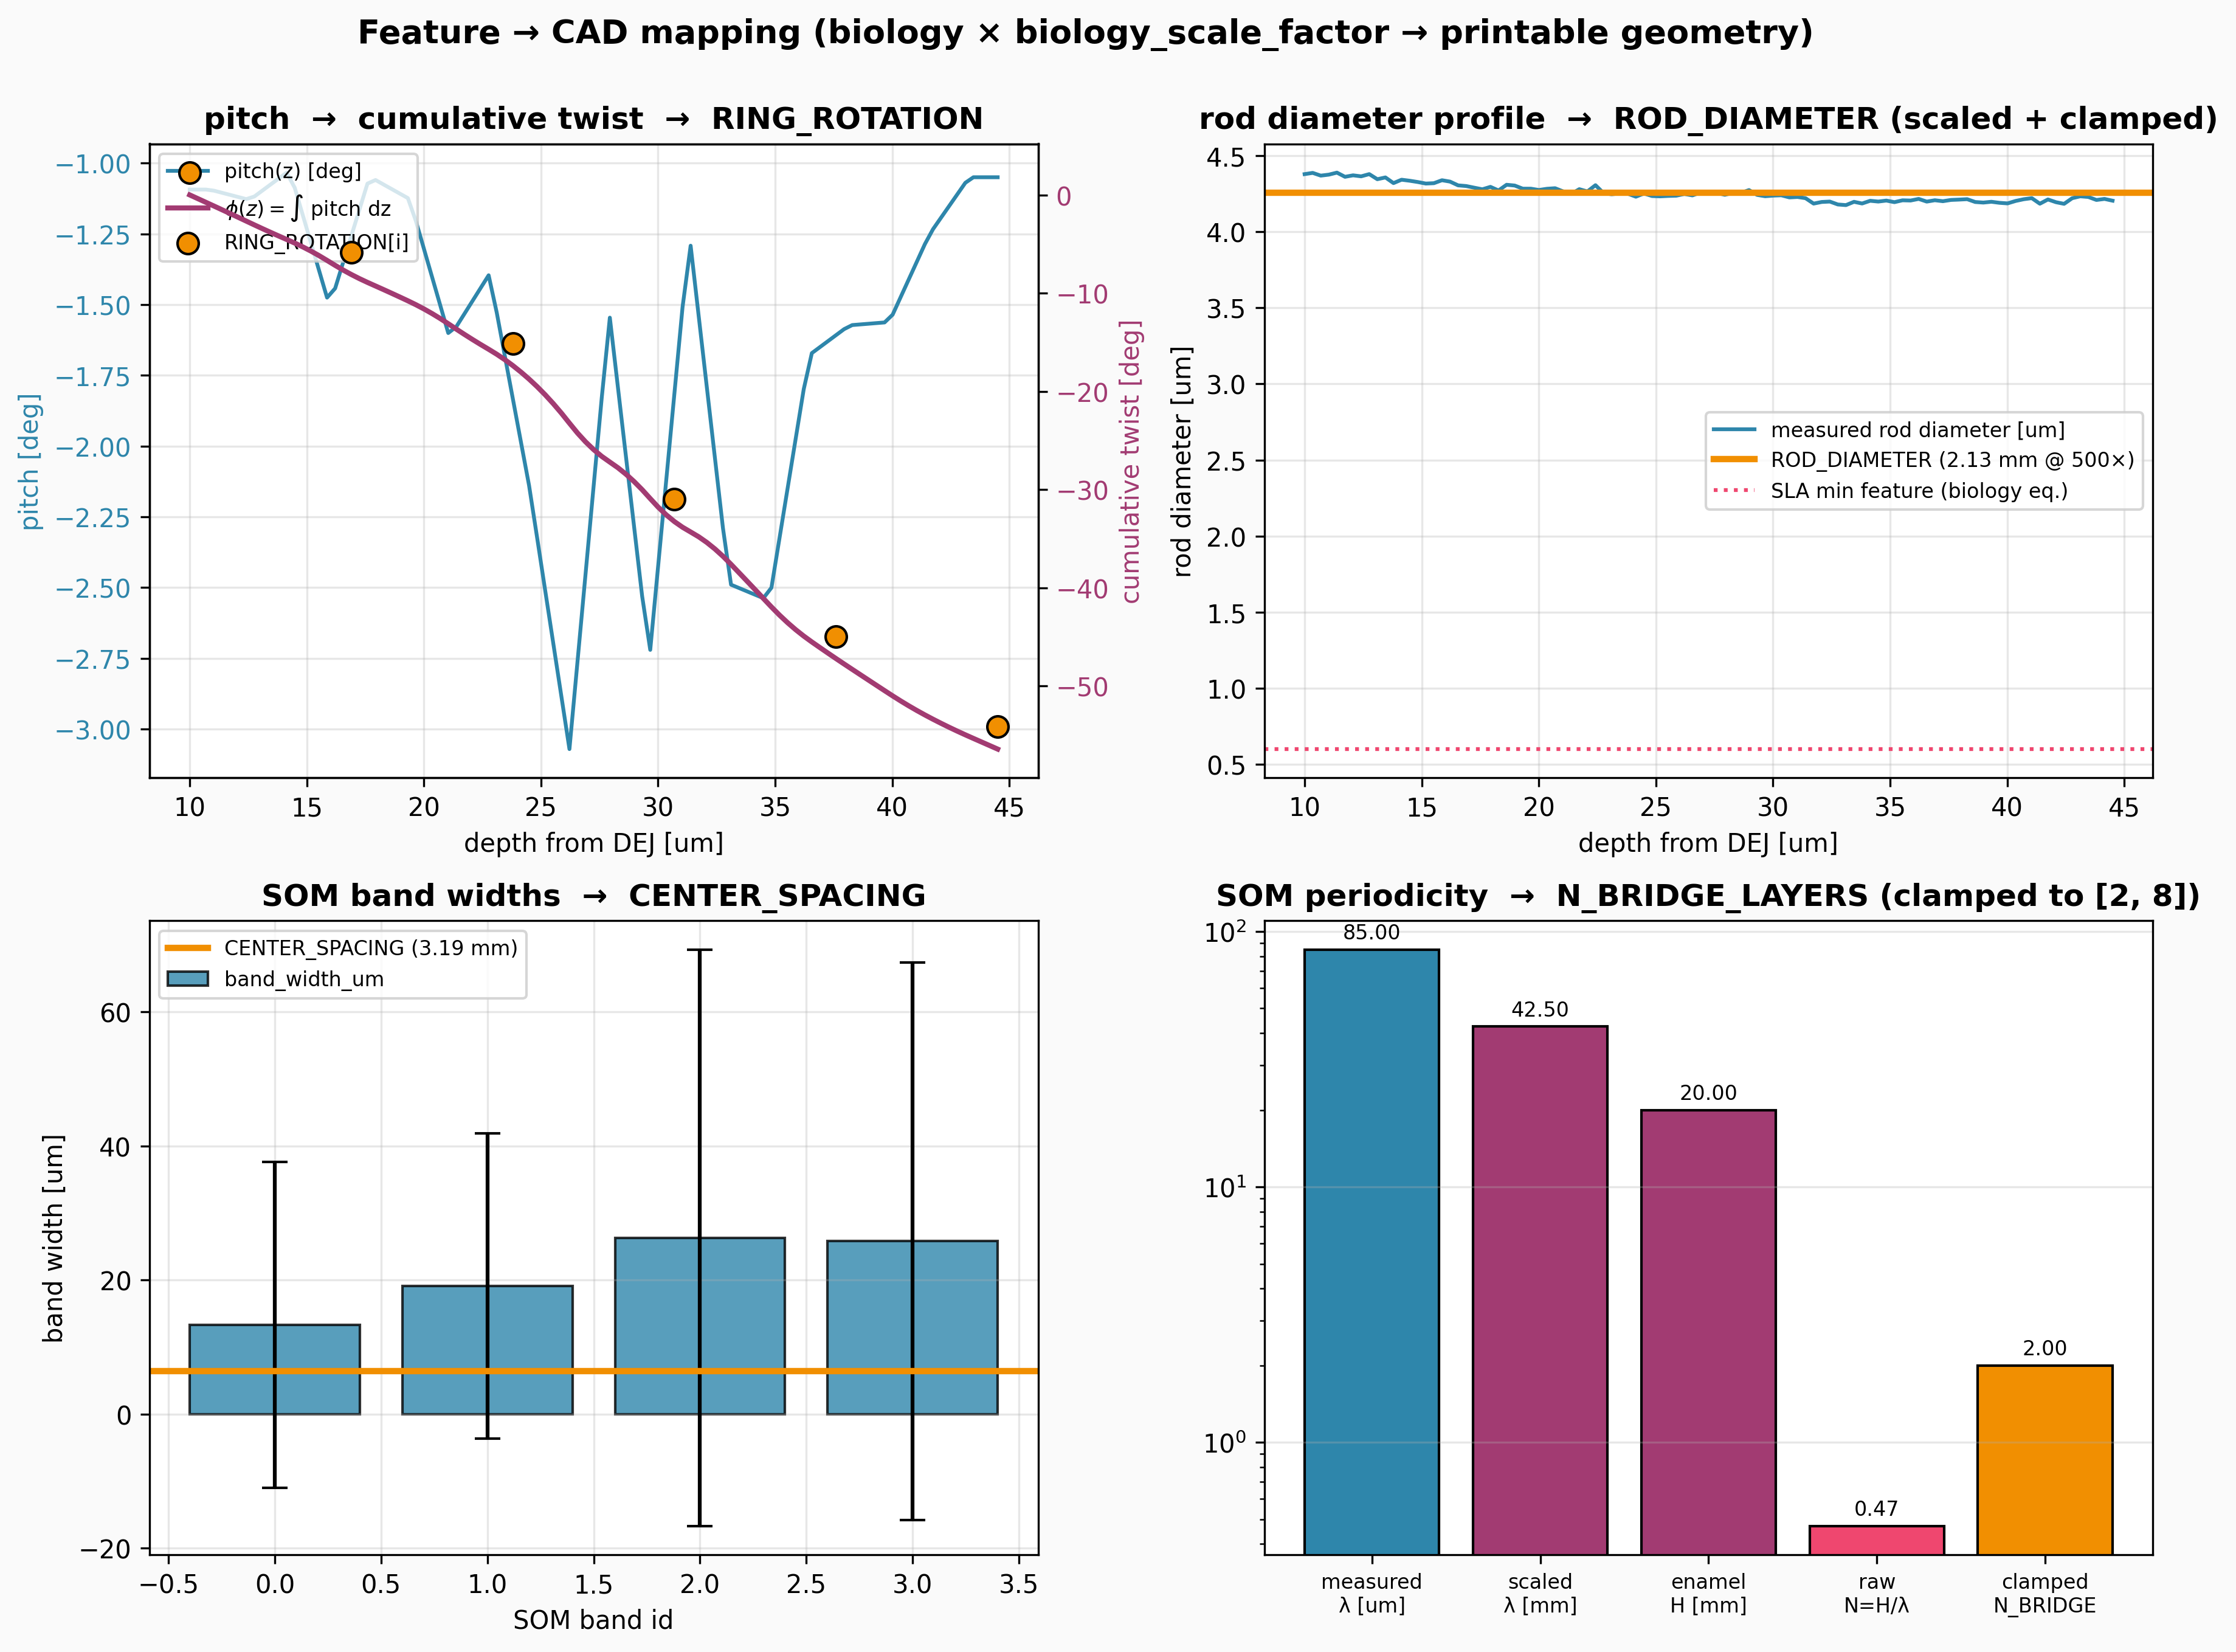
\includegraphics[width=0.98\linewidth]{figures/02_feature_to_cad.png}
\caption{Four representative feature-to-CAD mappings on the live specimen \texttt{enamel\_live\_001}. Top-left: signed pitch profile (blue) is integrated along $z$ to give the cumulative twist $\phi(z)$ (magenta); ring-specific values (orange markers) are interpolated onto the $N_{\text{rings}}+1$ nodes to populate \texttt{RING\_ROTATION}. Top-right: measured rod-diameter profile (blue), mean (dashed), and the SLA-clamped \texttt{ROD\_DIAMETER} back-converted to biology units (orange), relative to the SLA floor (pink dotted). Bottom-left: SOM band widths per band with mean superimposed as the mapped \texttt{CENTER\_SPACING}. Bottom-right: dominant wavelength scaled and divided into \texttt{ENAMEL\_THICKNESS} to derive the raw bridge-layer count, then clamped to $[2, 8]$.}
\label{fig:feat2cad}
\end{figure}

\subsection{Pitch profile $\to$ \texttt{RING\_ROTATION}}

Integrating the signed pitch along $z$ gives cumulative twist $\phi(z) = \int p(z)\,dz$ in degrees. This is resampled onto the ring nodes evenly spaced over \texttt{ENAMEL\_THICKNESS}. A shape classifier fits $\phi(z)$ against three canonical twist profiles (linear, accelerating, sigmoid) and picks the lowest RMSE. If no canonical shape fits within a 10\% residual, \texttt{TWIST\_TYPE} is set to \texttt{measured} and the full $(z, \phi)$ samples are stored in \texttt{measured\_twist\_profile} for the \texttt{measured\_profile\_twist} generator to consume as a CubicSpline.

\subsection{SOM band morphometrics $\to$ bridge geometry}

\begin{itemize}
  \item \textbf{Number of bridge layers} $N_{\text{bridge}} = \mathrm{clip}\bigl(\mathrm{round}(\text{ENAMEL\_THICKNESS} / \lambda_{\text{mm}}),\; 2,\; 8\bigr)$, where $\lambda_{\text{mm}}$ is the dominant SOM wavelength scaled by \texttt{biology\_scale\_factor}.
  \item \textbf{Anchor of \texttt{RING\_ROTATION}$[0]$} = mean direction of band~0, so the bottom ring aligns with the dominant measured band.
  \item \textbf{Center spacing}: mean \texttt{band\_width\_um} scaled and clamped as described in \S\,2.4.
\end{itemize}

\subsection{Rod morphometry $\to$ \texttt{ROD\_DIAMETER}, \texttt{ROD\_TAPER}, \texttt{per\_ring\_diameter}}

Mean measured rod diameter drives \texttt{ROD\_DIAMETER}. The fractional end-to-end difference $(d_{\text{top}} - d_{\text{bot}})/d_{\text{mid}}$ drives \texttt{ROD\_TAPER\_FACTOR}. If the diameter profile has more than 15\% non-monotone segments, the mapping emits a \texttt{per\_ring\_diameter} dictionary and routes the run through the \texttt{radially\_graded} generator. Mean eccentricity above 0.2 triggers an elliptical cross-section flag (consumed by a future stochastic-lattice variant).

\subsection{Tortuosity $\to$ \texttt{twist\_perturbation\_amplitude\_deg}}

Measured rod tortuosity above unity drives a proportional wobble amplitude (clipped to $[0, 15]$ degrees) consumed by the \texttt{hierarchical\_twist} generator to add fast rod-level perturbations on top of the slow ring-level twist. Wobble frequency is set from the SOM dominant wavelength.

% ============================================================
\section{FEA --- Strain Solver and Load-Normalised Metrics}
% ============================================================

Stock \texttt{compression\_test.py} is a prescribed-displacement linear-elasticity problem. The pipeline does not prescribe displacement; it solves for the displacement that produces a target representative stress.

\begin{figure}[h!]
\centering
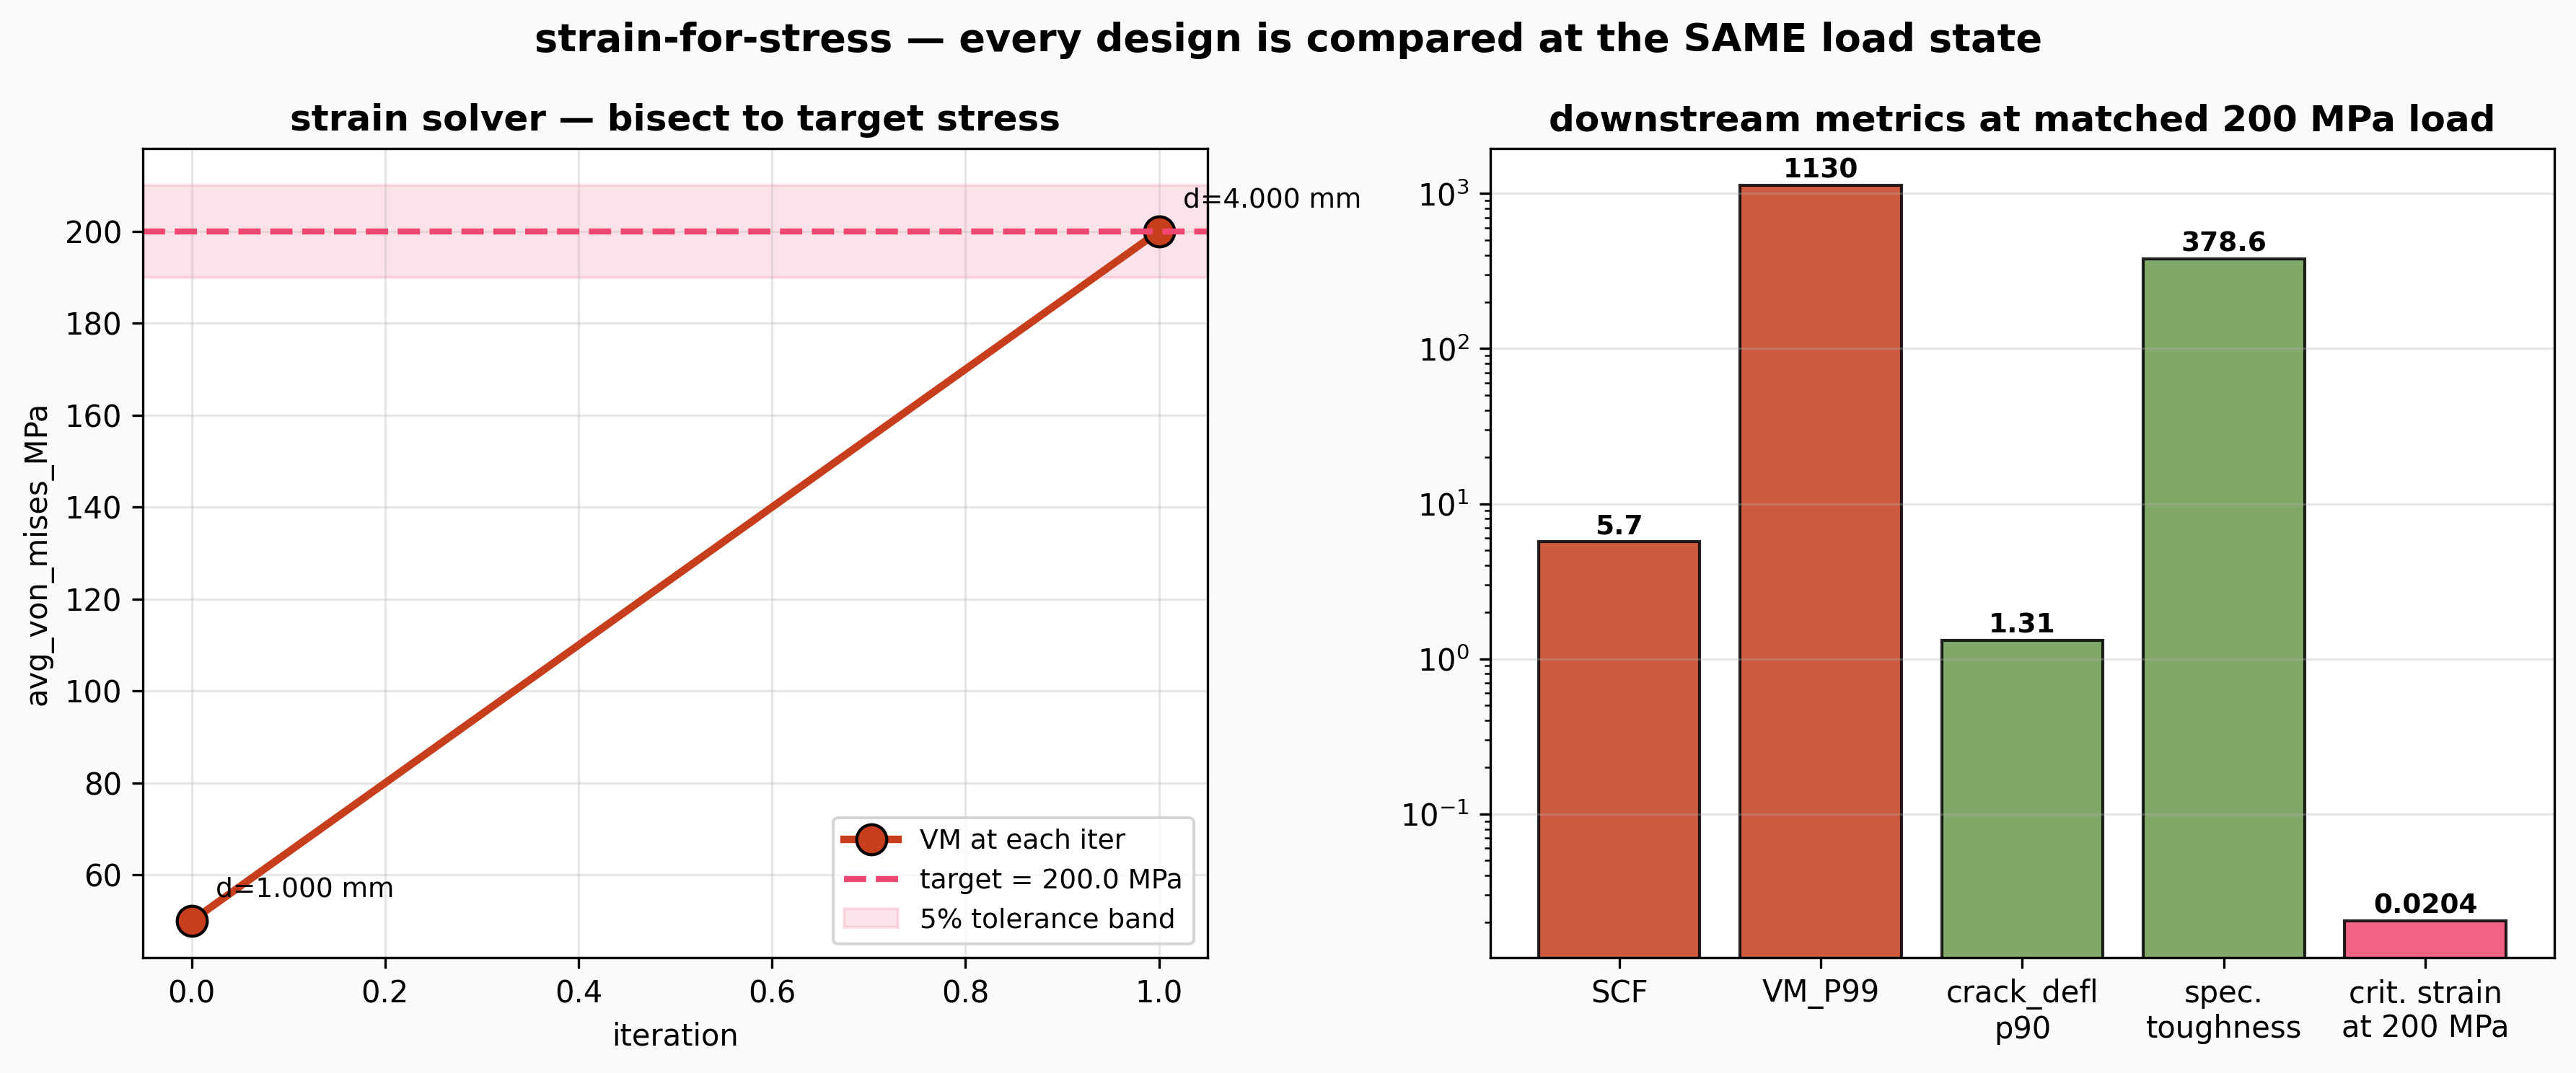
\includegraphics[width=0.98\linewidth]{figures/03_strain_solver.png}
\caption{Strain-for-stress strategy. Left: linear elasticity guarantees a single-iteration correction --- applied displacement scales as $d \leftarrow d \cdot \text{target}/\text{VM}$. A 5\% tolerance band is accepted; at most five iterations are allowed before falling back to a soft penalty. Right: every downstream metric (stress concentration, crack deflection, specific toughness, critical strain) is then evaluated at the same representative-load state across all designs.}
\label{fig:strain}
\end{figure}

\begin{mechanismbox}
\textbf{Algorithm.} Seed $d = d_0$. Run FEA; read \texttt{avg\_von\_mises\_MPa} (or \texttt{VM\_P50\_MPa}, computed volume-weighted from \texttt{element\_results\_compression.csv}). If $\lvert \mathrm{VM} - 200 \rvert / 200 \leq \text{tol}$, accept. Otherwise $d \leftarrow d \cdot (200/\mathrm{VM})$ and re-run. The mesh is held fixed across inner iterations --- only \texttt{COMPRESS\_DISP\_MM} changes. Record $\texttt{critical\_strain\_at\_200MPa} = \texttt{critical\_disp\_mm} / \texttt{specimen\_height\_mm}$.
\end{mechanismbox}

\subsection{Crack-deflection metric}

\begin{figure}[h!]
\centering
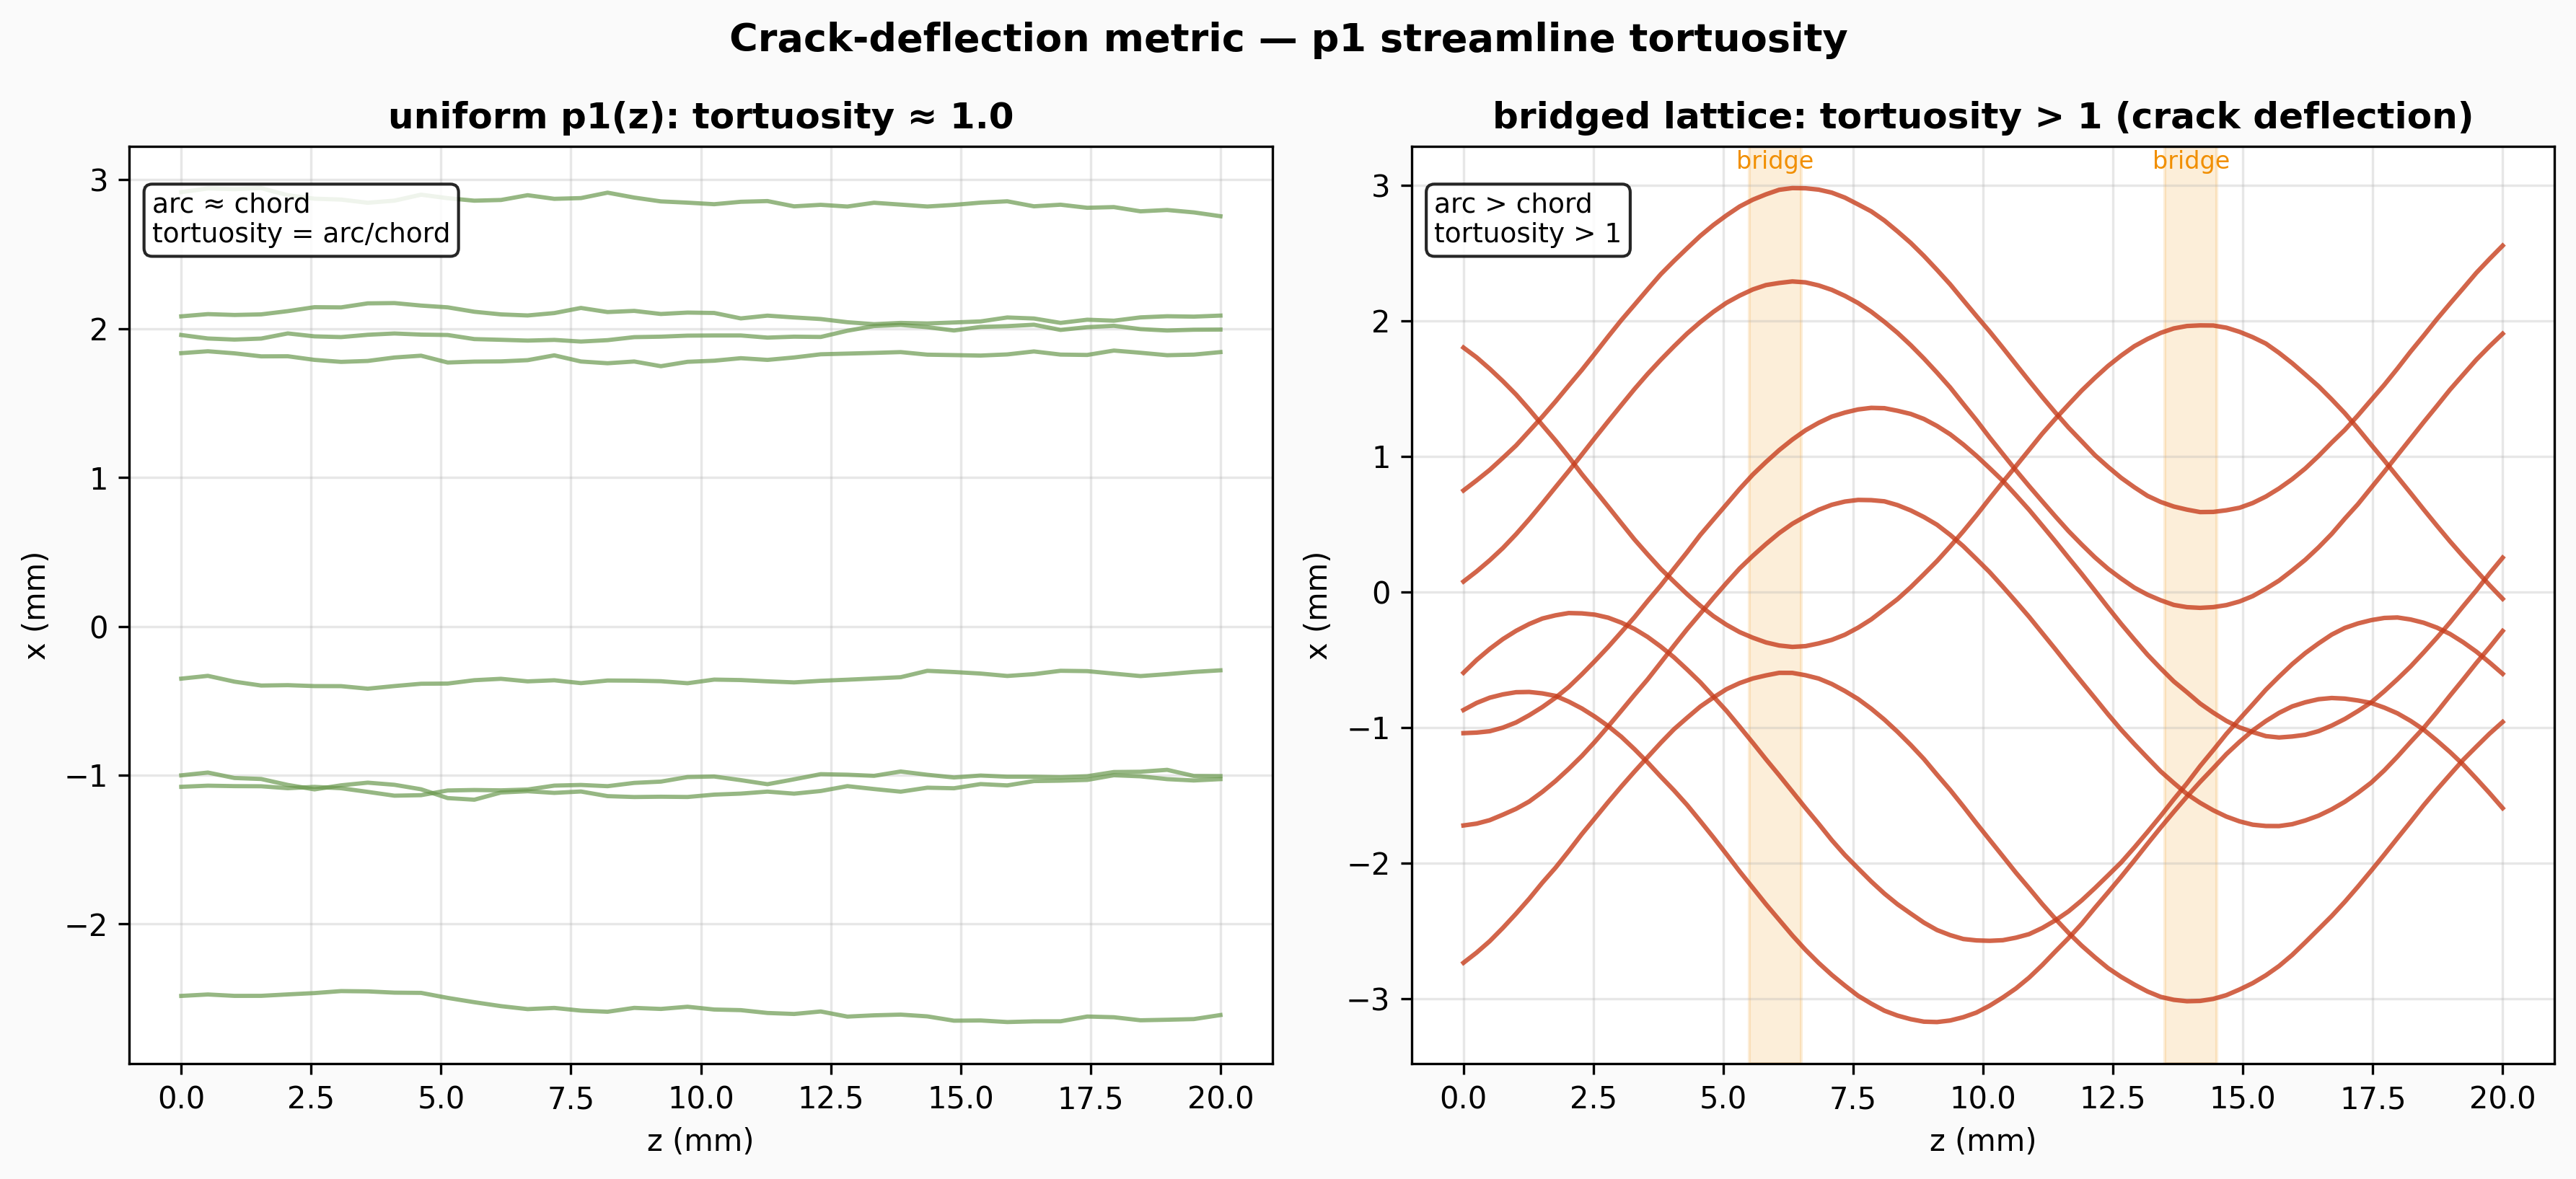
\includegraphics[width=0.98\linewidth]{figures/04_crack_deflection.png}
\caption{Crack-deflection metric: post-hoc streamline tortuosity of the max-principal-stress field. Left: in a uniform vertical $p_1(z)$ field, streamlines are straight and tortuosity $\approx 1$. Right: in the bridged lattice, the bridge bands force streamlines to deflect laterally, increasing the arc-to-chord ratio. The same arc-over-chord formula is used in \texttt{compute\_tortuosity.py} for the biological rod centerlines, so FEA and biology tortuosity are numerically comparable.}
\label{fig:crack}
\end{figure}

The implementation rasterises per-element \texttt{p1\_MPa} onto a 32$^3$ regular grid, computes the gradient field (with sign reoriented to $+z$), seeds 64 streamlines on the bottom face, and integrates each to the top face. Reported scalars are the mean, 90th percentile, and maximum of $\text{arc\_length}/\text{chord\_length}$ across streamlines, alongside the effective streamline count.

\subsection{Biomimicry score}

A z-scored Euclidean distance across five feature pairs (rod diameter, centre spacing, equivalent bridge-layer count, band-0 direction, tortuosity). Smaller values indicate a generated lattice closer to the measured biology.

% ============================================================
\section{Objective Registry}
% ============================================================

Every YAML under \texttt{config/objectives/} becomes a loadable \texttt{Objective} with a callable \texttt{.score(metrics\_dict)} $\to$ \texttt{float} and a \texttt{direction} flag. A \texttt{stress\_target} block drives the strain solver, so every objective is load-normalised by construction. Five are shipped:

\begin{table}[h!]
\centering
\caption{Built-in objective configurations.}
\label{tab:objectives}
\small
\renewcommand{\arraystretch}{1.3}
\begin{tabularx}{\linewidth}{l l X}
\toprule
\textbf{Name} & \textbf{Direction} & \textbf{Key terms (weights)} \\
\midrule
\texttt{crack\_deflection} (default) & maximize & \texttt{tortuosity\_p90} (1.0) + $\tfrac{1}{2}$\,\texttt{tortuosity\_mean} + $\tfrac{1}{4}$\,\texttt{critical\_strain\_at\_200MPa} \\
\texttt{toughness}                   & maximize & \texttt{specific\_toughness\_mJ\_per\_MPa} (1.0) + $0.1$\,\texttt{energy\_absorption\_mJ} \\
\texttt{stiffness\_target}           & minimize & $\lvert E_{\text{eff}} - 50\,\text{GPa} \rvert$ \\
\texttt{biomimicry\_score}           & minimize & \texttt{biomimicry\_score} (1.0) \\
\texttt{composite}                   & maximize & $1.0$\,\texttt{tortuosity\_p90} + $0.01$\,\texttt{toughness} $- 0.1$\,\texttt{SCF} \\
\bottomrule
\end{tabularx}
\end{table}

% ============================================================
\section{Closed-Loop Biomimicry}
% ============================================================

\begin{figure}[h!]
\centering
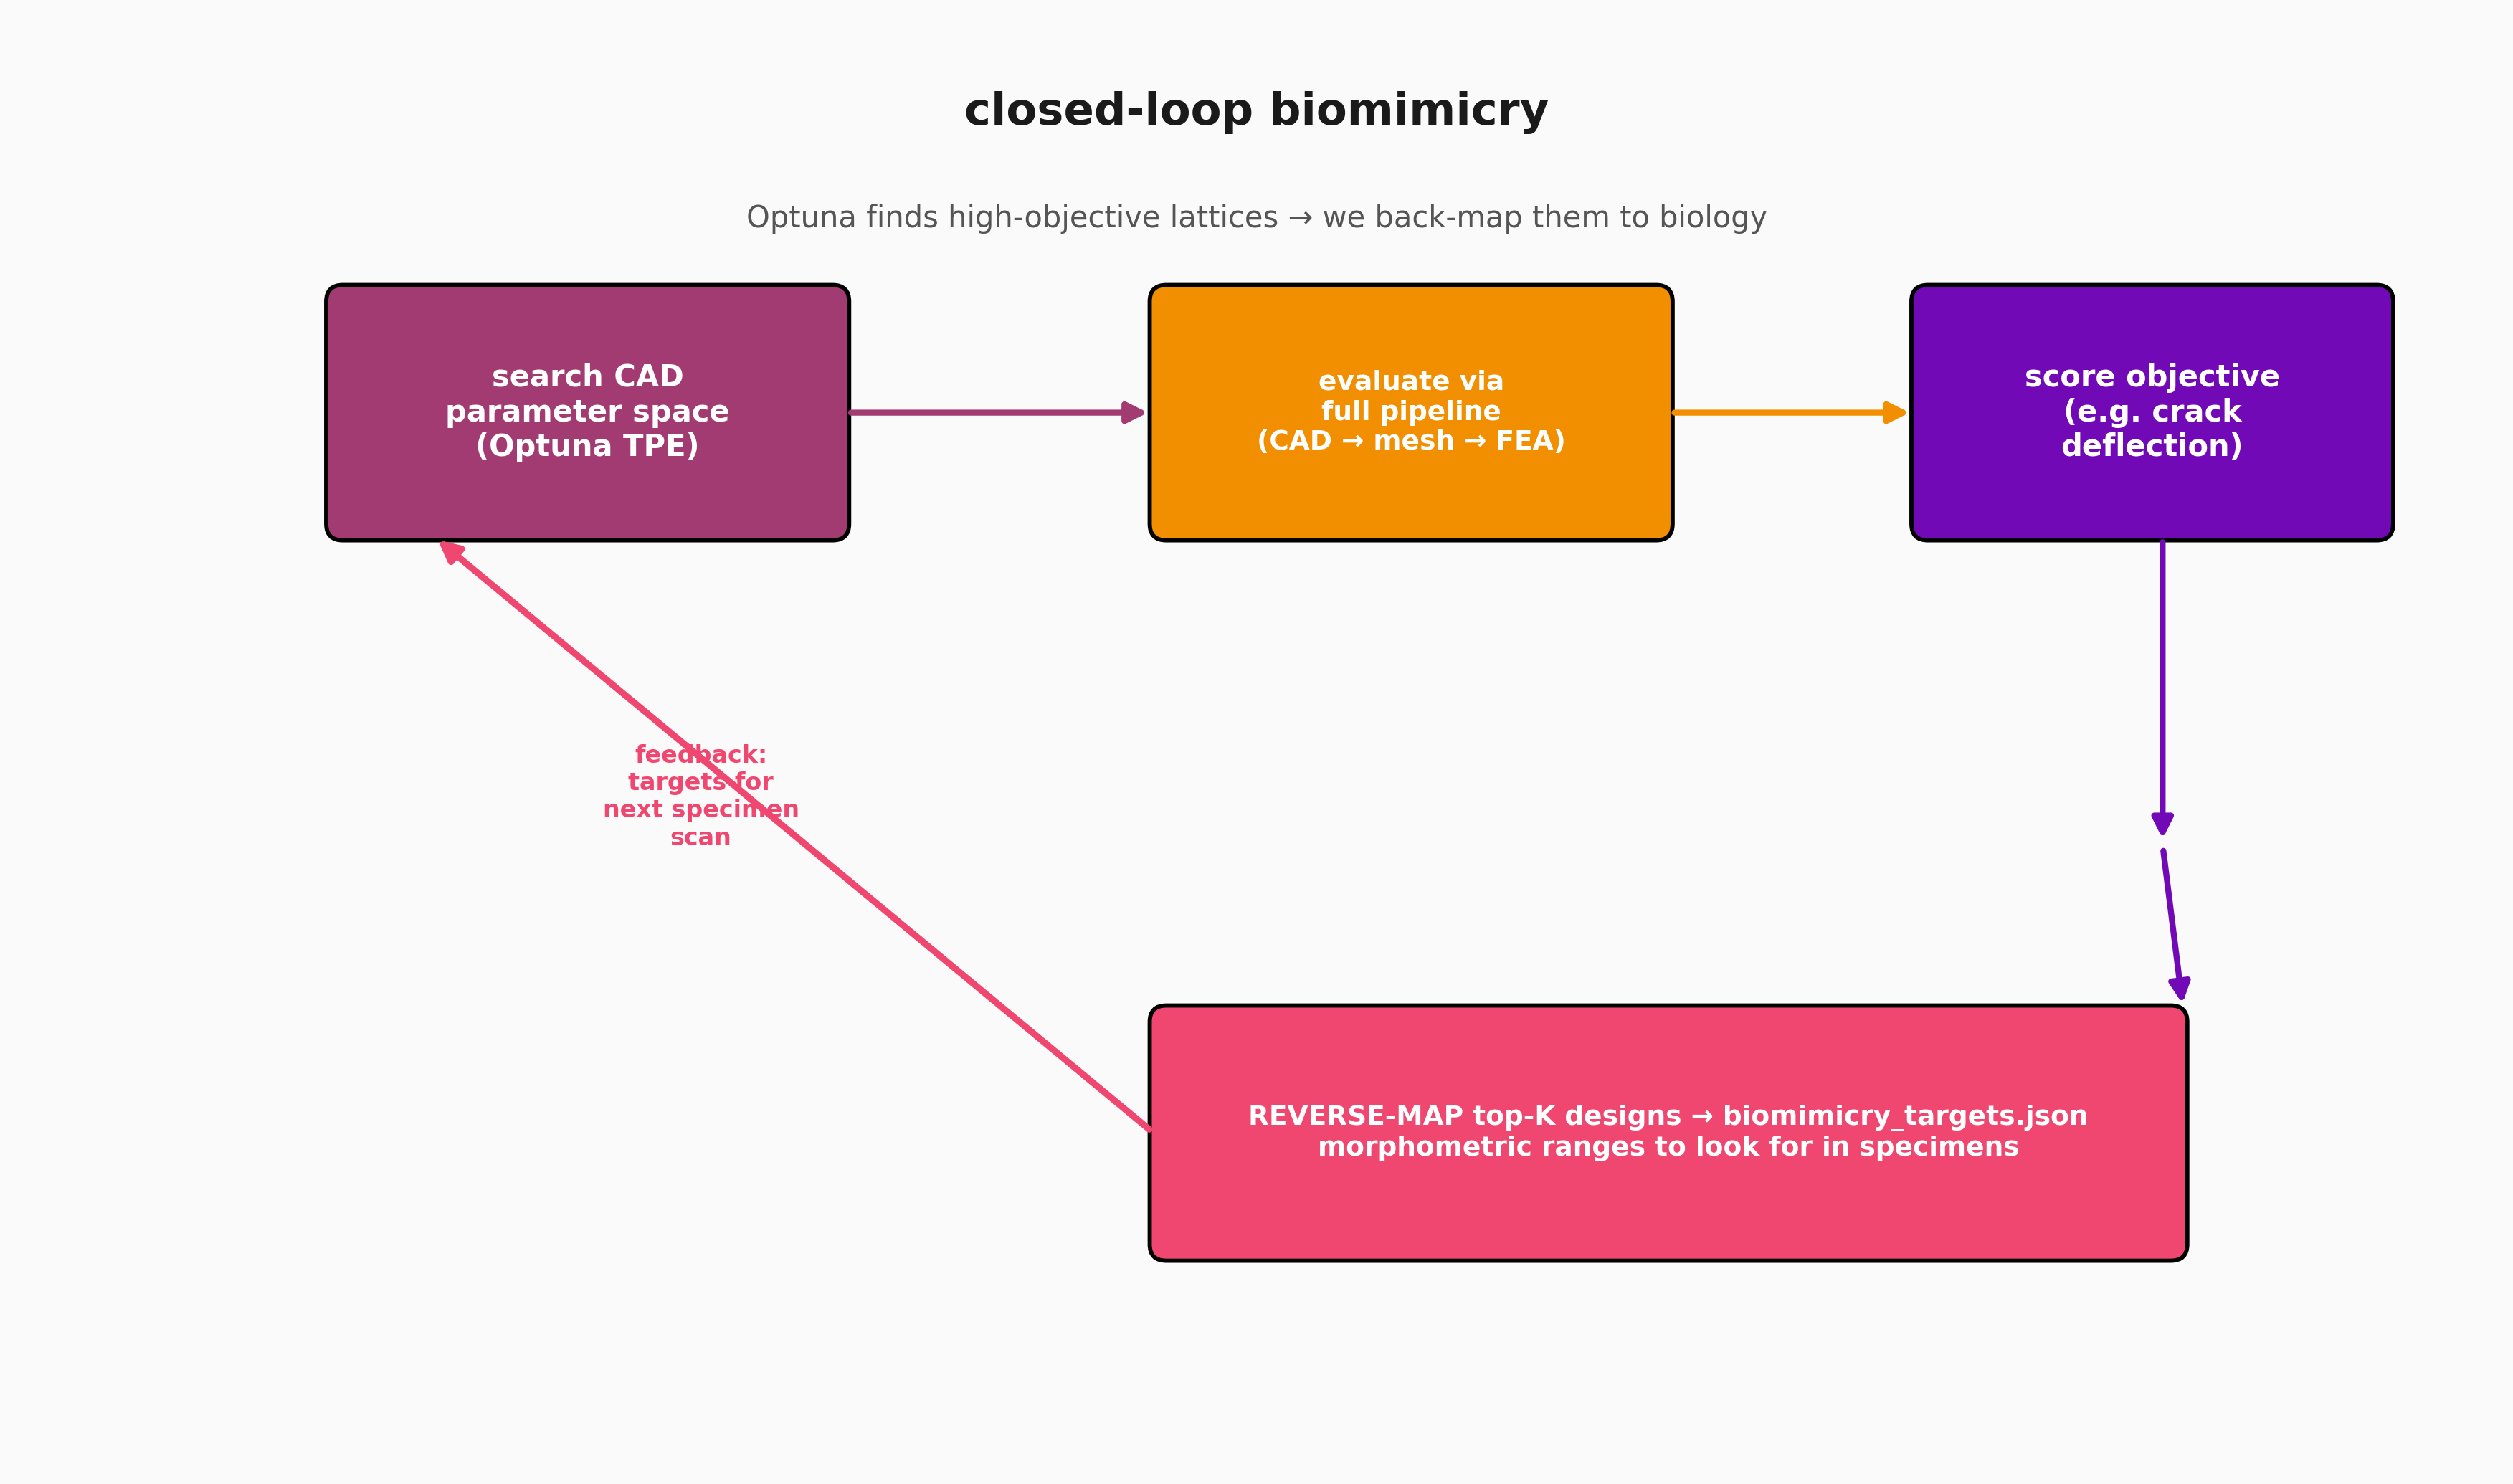
\includegraphics[width=0.92\linewidth]{figures/05_closed_loop.png}
\caption{Closed-loop biomimicry (stage~3 deliverable). An unconstrained Optuna TPE search scans the full CAD parameter space, evaluating each candidate via the full digital-twin pipeline. The top-$K$ designs are reverse-mapped back into morphometric ranges --- these are the measurable features biology would need to exhibit to produce similarly high-objective lattices. The output file \texttt{biomimicry\_targets.json} names those ranges so field work can prioritise specimens with the target morphometrics.}
\label{fig:closedloop}
\end{figure}

\begin{conclusionbox}{Reverse-map applied to top-$K$ CAD designs}
\begin{itemize}
  \item $\texttt{ROD\_DIAMETER} \times 10^3 / \texttt{biology\_scale\_factor} \to $ rod diameter in $\si{\micro\meter}$
  \item $\texttt{CENTER\_SPACING} \times 10^3 / \texttt{biology\_scale\_factor} \to $ SOM band width in $\si{\micro\meter}$
  \item $\texttt{ENAMEL\_THICKNESS} / \texttt{N\_BRIDGE\_LAYERS} / \texttt{biology\_scale\_factor} \times 10^3 \to $ dominant wavelength in $\si{\micro\meter}$
  \item $\texttt{RING\_ROTATION}[0] \to $ band-0 mean direction in degrees
\end{itemize}
Summarised as $\{\text{mean}, \text{min}, \text{max}\}$ per feature across top-$K$, plus a categorical mode for \texttt{TWIST\_TYPE}.
\end{conclusionbox}

% ============================================================
\section{Per-Run Output Tree}
% ============================================================

\begin{figure}[h!]
\centering
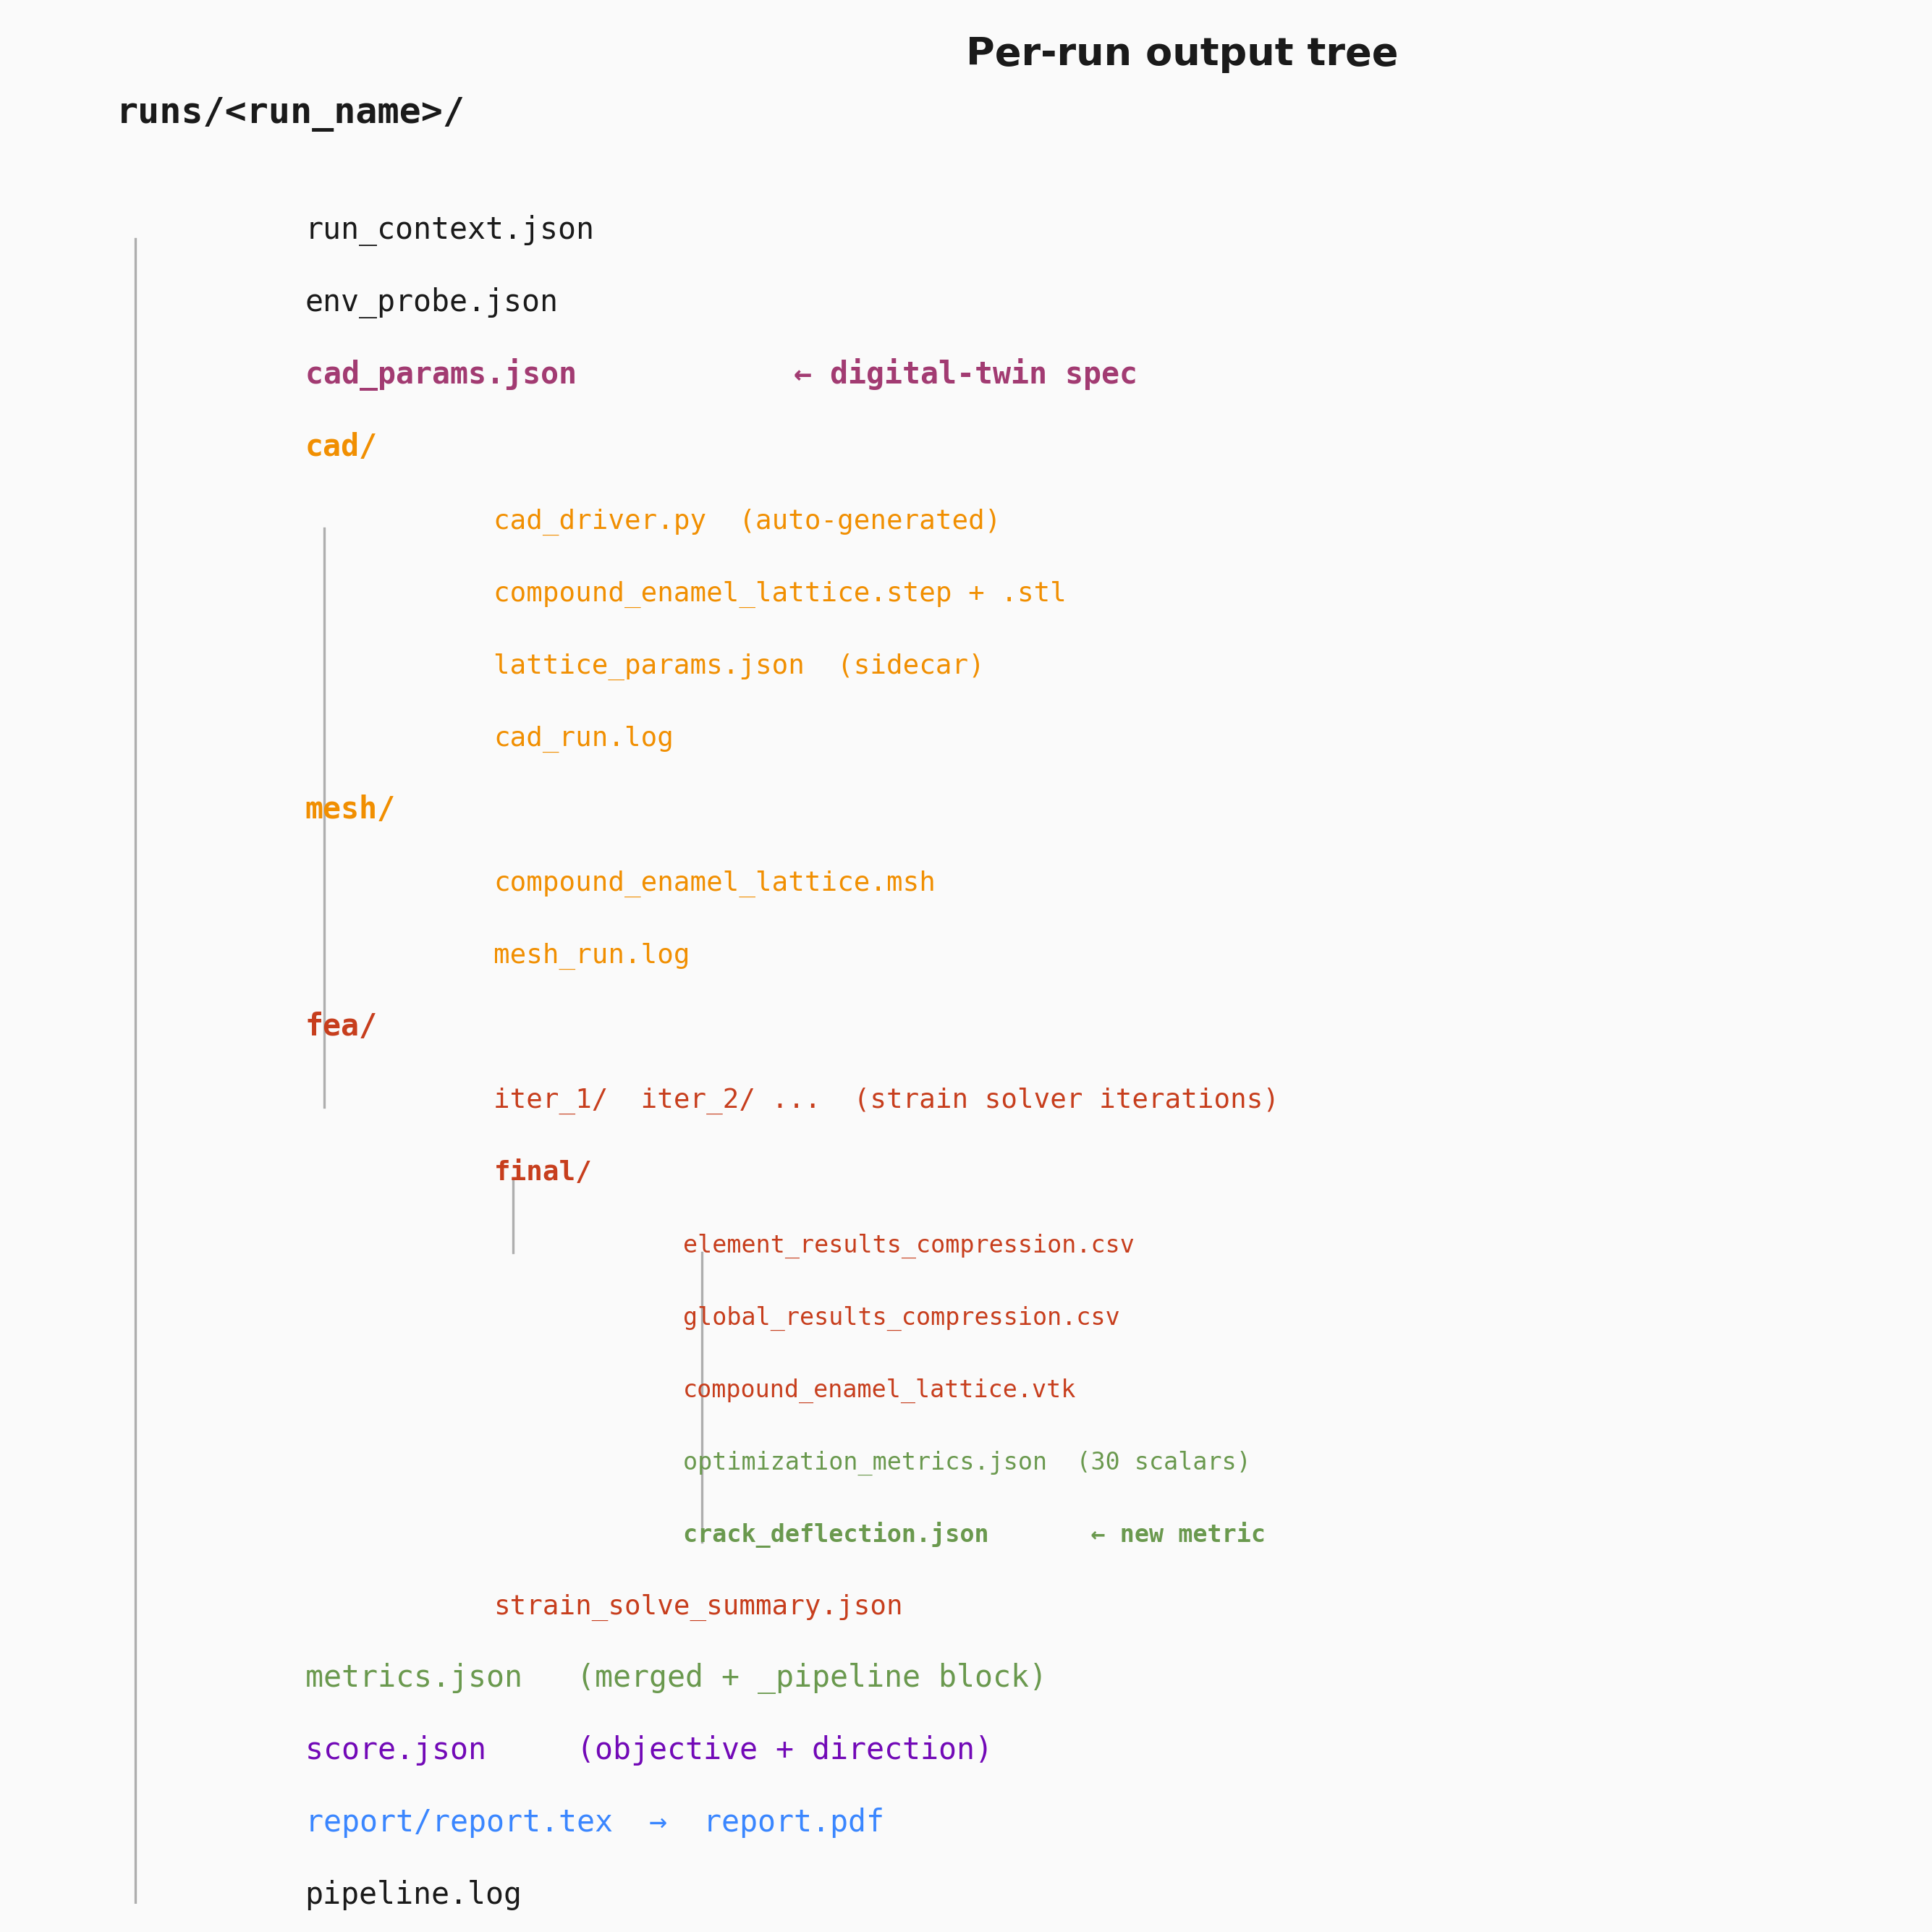
\includegraphics[width=0.85\linewidth]{figures/06_run_tree.png}
\caption{Annotated output tree produced by \texttt{scripts/run\_pipeline.py} for a single specimen. The per-iteration FEA working directories (\texttt{iter\_1/}, \texttt{iter\_2/}, \ldots) hold full per-element and per-vertex data; the accepted iteration is promoted to \texttt{final/} and \texttt{extract\_metrics.py} is run there. \texttt{crack\_deflection.json} is added by the new post-hoc metric module; \texttt{metrics.json} is the merged superset used to score the objective.}
\label{fig:runtree}
\end{figure}

% ============================================================
\section{Live Validation Run}
% ============================================================

A live end-to-end execution was performed on the specimen \texttt{enamel\_live\_001} (the 100-slice microCT stack under \texttt{output\_validation\_100/}, \texttt{output\_hsb\_roi/}, \texttt{output\_piv/}, and \texttt{som\_approach/output\_som\_morphometrics/}). Total wall time on an Apple Silicon MacBook Pro was $\approx 9$\,min\,17\,s.

\begin{table}[h!]
\centering
\caption{Live-run timing breakdown (specimen \texttt{enamel\_live\_001}).}
\label{tab:timing}
\small
\renewcommand{\arraystretch}{1.3}
\begin{tabularx}{\linewidth}{l l X}
\toprule
\textbf{Stage} & \textbf{Wall time} & \textbf{Output} \\
\midrule
Ingest \& merge      & $< 1$\,s  & \texttt{morphometrics.json} (6 sources, sha256 provenance) \\
Map                  & $< 1$\,s  & \texttt{cad\_params.json} (9 logged clamps, all audited) \\
CAD                  & $64$\,s   & 91 rods, 180 bridges, $15$\,MB STEP, $67$\,MB STL \\
Mesh                 & $20$\,s   & $947$\,k tets, $62$\,MB MSH \\
Strain solver        & $7$\,min\,$45$\,s & 2 iterations; $d{=}4.92$\,mm $\to$ $\overline{\mathrm{VM}}{=}200.00$\,MPa exactly \\
Metrics extraction   & $3$\,s    & 30 stock scalars in \texttt{optimization\_metrics.json} \\
Crack deflection     & $4$\,s    & 64 streamlines; mean$=2.30$, p90$=7.09$, max$=9.14$ \\
Biomimicry           & $<1$\,s   & score $= 0.57$ over 5 feature pairs \\
Report               & $<1$\,s   & \texttt{report.tex} $\to$ \texttt{report.pdf} \\
\bottomrule
\end{tabularx}
\end{table}

\begin{table}[h!]
\centering
\caption{Key metrics from the live specimen \texttt{enamel\_live\_001} at the matched 200\,MPa load state.}
\label{tab:livemetrics}
\small
\renewcommand{\arraystretch}{1.3}
\begin{tabular}{l r l}
\toprule
\textbf{Metric} & \textbf{Value} & \textbf{Interpretation} \\
\midrule
\texttt{critical\_strain\_at\_200MPa}         & $0.2245$    & 22.4\% compressive strain to reach 200\,MPa \\
\texttt{critical\_disp\_mm\_at\_200MPa}       & $4.916$\,mm & absolute displacement at target stress \\
\texttt{E\_effective\_MPa}                    & $614$       & effective modulus at print-scale \\
\texttt{SCF}                                  & $8.91$      & stress concentration factor \\
\texttt{VM\_P50\_MPa}                         & $108.1$     & median von-Mises at critical load \\
\texttt{VM\_P99\_MPa}                         & $797.7$     & tail of VM distribution \\
\texttt{specific\_toughness\_mJ\_per\_MPa}    & $105.4$     & volumetric toughness index \\
\texttt{crack\_deflection\_tortuosity\_mean}  & $2.30$      & mean streamline arc/chord \\
\texttt{crack\_deflection\_tortuosity\_p90}   & $7.09$      & 90th percentile crack deflection \\
\texttt{crack\_deflection\_tortuosity\_max}   & $9.14$      & worst-case crack deflection \\
\texttt{biomimicry\_score}                    & $0.569$     & distance to measured biology (lower is closer) \\
\textbf{objective score (crack\_deflection)}  & $\mathbf{8.29}$ & composite of p90, mean, critical strain \\
\bottomrule
\end{tabular}
\end{table}

\begin{mechanismbox}
\textbf{Notable fixes that landed during live validation.}
\begin{enumerate}
  \item Separated \texttt{gmsh} probe target into \texttt{sfepy\_env} (the stock pipeline also runs Gmsh there; \texttt{cad\_env} only has CadQuery).
  \item Subprocess wrapper now passes \texttt{[python, script, \ldots]} to \texttt{conda run} (previously stripped the \texttt{python} argument, which caused \texttt{conda run} to try to exec the \texttt{.py} directly --- rc~126).
  \item Mesh runner uses \texttt{sfepy\_env} primary with \texttt{cad\_env} fallback, matching stock \texttt{optimize\_lattice.py:171}.
  \item Bridge-placement safe zone expanded to account for the junction sphere radius, not just the bridge half-diameter; previously the junction spheres at the bottom bridge overlapped the bottom plate and produced a degenerate OCC topology that Gmsh reported as ``PLC Error: segment and facet intersect.''
  \item FEA runner now copies the stock \texttt{compression\_test.py} into the per-iteration working directory; \texttt{sfepy-run} changes CWD to the problem-def script's parent dir, which previously caused the relative mesh path (\texttt{compound\_enamel\_lattice.msh}) to resolve to a stale mesh sitting next to the stock script rather than our freshly generated mesh.
  \item Per-run LaTeX report now escapes LaTeX-special characters (\texttt{\_}, \texttt{\&}, \texttt{\%}, \texttt{\$}, \ldots) before substitution so arbitrary specimen IDs and run names render without triggering math-mode errors.
\end{enumerate}
\end{mechanismbox}

% ============================================================
\section{CLI Reference}
% ============================================================

All scripts live under \texttt{biomimetic\_pipeline/scripts/} and can be invoked as \texttt{python -m scripts.\textit{name}} from the project root, or \texttt{python scripts/\textit{name}.py}.

\subsection{Ingest features}
\begin{lstlisting}
python scripts/ingest_features.py \
    --specimen-id enamel_001 \
    --out runs/ingest_001/morphometrics.json \
    [--no-validate]
\end{lstlisting}

\subsection{Generate CAD only (no mesh/FEA)}
\begin{lstlisting}
python scripts/generate_cad.py \
    --morphometrics runs/ingest_001/morphometrics.json \
    --export-dir runs/cad_only_001 \
    [--model-type {continuous_twist|measured_profile|hierarchical|radially_graded}]
\end{lstlisting}

\subsection{Full digital-twin pipeline}
\begin{lstlisting}
python scripts/run_pipeline.py \
    --morphometrics runs/ingest_001/morphometrics.json \
    --run-name digital_twin_001 \
    --objective crack_deflection \
    --model-type continuous_twist \
    [--material-E-mpa 3000] [--material-nu 0.40] \
    [--mesh-size-mm 0.5] [--junction-refinement 0.5]
\end{lstlisting}

\subsection{Parametric sweep}
\begin{lstlisting}
python scripts/run_sweep.py \
    --morphometrics runs/ingest_001/morphometrics.json \
    --run-name sweep_bridge_diameter \
    --param BRIDGE_DIAMETER --values 0.5 0.75 1.0 1.25 1.5 \
    --objective crack_deflection
\end{lstlisting}

\subsection{Optuna Bayesian optimisation}
\begin{lstlisting}
python scripts/run_optimize.py \
    --morphometrics runs/ingest_001/morphometrics.json \
    --run-name opt_cd_001 \
    --objective crack_deflection --n-trials 30 [--seed 42]
\end{lstlisting}

\subsection{Closed-loop biomimicry reverse-map}
\begin{lstlisting}
python scripts/run_closed_loop.py \
    --run-name closed_cd_001 \
    --objective crack_deflection \
    --n-trials 30 --top-k 5
\end{lstlisting}

% ============================================================
\section{Verification}
% ============================================================

\texttt{python tests/run\_all.py} runs five unit-test modules --- none requires \texttt{cad\_env} or \texttt{sfepy\_env}.

\begin{table}[h!]
\centering
\caption{Unit-test coverage.}
\label{tab:tests}
\small
\renewcommand{\arraystretch}{1.25}
\begin{tabularx}{\linewidth}{l X}
\toprule
\textbf{Module} & \textbf{What it proves} \\
\midrule
\texttt{test\_strain\_solver.py}    & Linear FEA converges in 1 iter; mild non-linearity within 5; summary JSON persisted \\
\texttt{test\_crack\_deflection.py} & Uniform $p_1(z) = z$ $\to$ tortuosity $\approx 1.0$; radial-bowl field bends paths into $[1, 2]$ \\
\texttt{test\_mapping.py}           & Monotone pitch $\to$ monotone \texttt{RING\_ROTATION}; clamps logged; eccentricity $> 0.2$ $\to$ ellipse; non-monotone diameter $\to$ \texttt{per\_ring\_diameter} populated \\
\texttt{test\_new\_models.py}       & Measured-profile twist returns 0 at $z=0$ and total-rotation at $z=H$; hierarchical wobble adds correctly at $z=H/4$ \\
\texttt{test\_objective\_registry.py} & All five YAMLs load; \texttt{crack\_deflection} is monotone in tortuosity; off-target penalty applied \\
\bottomrule
\end{tabularx}
\end{table}

% ============================================================
\section{Limitations \& Next Steps}
% ============================================================

\begin{limitbox}
\textbf{Known limitations (as of April 14, 2026).}
\begin{itemize}
  \item The stock meshing chain still emits a ``PLC error'' on some tight-geometry parameter combinations; this is upstream of the pipeline and must be resolved in \texttt{lattice\_cad.py} / Gmsh. The sphere-aware safe-zone clamp in mapping mitigates the common case.
  \item Phase-4 \texttt{radially\_graded} uses the mean of \texttt{per\_ring\_diameter}; true per-ring variation requires dropping the hexagonal grid generator in \texttt{lattice\_cad.py}, which is scheduled for Phase-5 (\texttt{stochastic\_lattice}).
  \item The \texttt{composite} objective weights are illustrative; the coefficients should be tuned by cross-validation against an independent held-out specimen before being used for production optimisation.
  \item Fatigue / cyclic loading is not currently in the stress-solver vocabulary; the strain-to-stress bisection assumes monotonic compression in the linear-elastic regime.
\end{itemize}
\end{limitbox}

\begin{conclusionbox}{Immediate next steps}
\begin{enumerate}
  \item Run \texttt{scripts/run\_sweep.py} over \texttt{BRIDGE\_DIAMETER} at $[0.5, 0.75, 1.0, 1.25, 1.5]$~mm to populate a first design-space map with the live specimen as the mapping seed.
  \item Run \texttt{scripts/run\_closed\_loop.py} with $N = 30$ trials and $K = 5$ to produce a first \texttt{biomimicry\_targets.json} --- i.e.\ the first biology-informed ``wanted poster'' of morphometric ranges to search for in new microCT cohorts.
  \item Port the \texttt{measured\_profile\_twist} generator to a full per-ring spline formulation so mapped lattices match the measured $\phi(z)$ directly instead of the closest canonical shape.
  \item Add a Phase-6 cross-validation harness: generate digital twins for three held-out specimens, compare simulated crack-deflection tortuosity against the biological rod-centerline tortuosity from PIV, and report pairwise correlation.
\end{enumerate}
\end{conclusionbox}

\end{document}
